
\section{Multi-class Recognition Policy} \label{sec:tech}

Our goal is a multi-class recognition policy $\pi$ that takes an image $\mathcal{I}$ and outputs a list of multi-class detection results by running detector and global scene \emph{actions} sequentially.

The policy repeatedly selects an action $a_i \in \mathcal{A}$, executes it, receiving observations $o_i$, and then selects the next action.
The set of actions $\mathcal{A}$ can include both classifiers and detectors: anything that would be useful for inferring the contents of the image.

Each action $a_i$ has an expected cost $c(a_i)$ of execution.
Depending on the setting, the cost can be defined in terms of algorithmic runtime analysis, an idealized property such as number of \emph{flops}, or simply the empirical runtime on specific hardware.
We take the empirical approach: every executed action advances $t$, the \emph{time into episode}, by its runtime.

As shown in Figure~\ref{fig:figure1}, the system is given two times: the setup time $T_s$ and deadline $T_d$.
From the setup time to the deadline, we want to obtain the best possible answer if stopped at any given time.
A single-number metric that corresponds to this objective is the area captured under the curve between the start and deadline bounds, normalized by the total area.
We evaluate policies by this more robust metric and not simply by the final performance at deadline time for the same reason that Average Precision is used instead of a fixed Precision vs. Recall point in the conventional evaluations.

\subsection{Sequential Execution}
An \emph{open-loop} policy takes actions in a sequence that does not depend on observations received from previous actions.
The common classifier cascade is an example \cite{Viola2001}.
In contrast, our goal is to learn a dynamic, or \emph{closed-loop}, policy, which would exploit the signal in scene and inter-object context for a maximally efficient path through the actions.

We refer to the information available to the decision process as the \emph{state} $s$.
The state includes the currently believed distribution over class presence variables $P(\mathbf{C}) = \{P(C_0), \ldots, P(C_K)\}$, where we write $P(C_k)$ to mean $P(C_k=1)$.

Additionally, the state records that an action $a_i$ has been taken by adding it to the initially empty set $\mathcal{O}$ and recording the resulting observations $o_i$.
We refer to the current set of observations as $\mathbf{o} = \{o_i | a_i \in \mathcal{O}\}$.
The state also keeps track of the time into episode $t$, and the setup and deadline times $T_s,T_d$.

A recognition \emph{episode} takes an image $\mathcal{I}$ and proceeds from the initial state $s^0$ and action $a^0$ to the next pair $(s^1,a^1)$, and so on until $(s^J,a^J)$, where $J$ is the last step of the process with $t \le T_d$.
At that point, the policy is terminated, and a new episode can begin on a new image.

The specific actions we consider in the following exposition are detector actions $a_{{det}_i}$, where ${det}_i$ is a detector class $C_i$, and a scene-level context action $a_{gist}$, which updates the probabilities of all classes.

\subsection{Selecting actions} \label{sec:value}
As our goal is to pick actions dynamically, we want a function $Q(s,a): S \times \mathcal{A} \mapsto \mathbb{R}$, where $S$ is the space of all possible states, to assign a value to a potential action $a \in \mathcal{A}$ given the current state $s$ of the decision process.
We can then define the desired policy $\pi$ as simply taking the (untaken) action with the maximum value:
\begin{align}
\pi(s) = \argmax_{a_i \in \mathcal{A} \setminus \mathcal{O}} Q(s,a_i)
\end{align}

Although the action space $\mathcal{A}$ is quite manageable, consisting of the detectors and global classifier we would like to run on the image, the space of possible states $S$ is intractable.
Therefore we cannot learn a tabular representation of $Q(s,a)$, and must use function approximation to represent it \cite{Sutton1998}.
We featurize the state-action pair and assume linear structure: $Q^\pi(s,a_i) = \theta_\pi^\top  \phi(s,a_i)$.

The policy's performance at time $t$ is determined by the detections that are part of the set of observations $\mathbf{o}^j$ at the last state $s^j$ before $t$.
Therefore, the final AP vs. Time evaluation of an episode is a function $eval(h,T_s,T_d)$ of the history of execution $h=s^0,s^1,\dots,s^J$.
It is precisely the normalized area under the AP vs. Time curve between $T_s$ and $T_d$, as determined by the detections in $\mathbf{o}^j$ for all steps $j$ in the episode.

As shown in \autoref{fig:rewards}, this evaluation function is additive per action, as each action can generate detections that either raise or lower the mean AP of the results so far ($\Delta ap$) and takes a certain time ($\Delta t$).
From these and $T_s$ and $T_d$, we can find the area under the curve that was contributed by the action.
So, we can then represent the final evaluation $eval(h,T_s,T_d)$ in terms of individual rewards: $\sum_{j=0}^J R(s^j,a^j)$.

Specifically, as shown in Figure~\ref{fig:rewards}, we define the \emph{reward} of an action as
\begin{align}\label{eq:advanced}
R(s^j,a_i) = \Delta \text{ap}_i (t_T^j-\frac{1}{2}\Delta t_i)
\end{align}
where $t_T^j$ and $\text{ap}^j$ are the time left until the deadline and the AP at state $s^j$, and $\Delta t_i$ and $\Delta \text{ap}_i$ are the time taken and AP change produced by the action $a_i$.
(For clarity of exposition, we do not account for $T_s$ here.)

\subsection{Learning the policy}
The expected value of the final evaluation can be written recursively in terms of the value function:
\begin{align} \label{eq:recursive_value}
Q^\pi(s^j,a_i) = \mathbb{E}_{s^{j+1}} [R(s^j,a_i) + \gamma Q^\pi(s^{j+1},\pi(s^{j+1}))]
\end{align}
where $\gamma \in [0,1]$ is a \emph{discount} value that can mitigate the effects of increasing state-transition uncertainty over long episodes.

While we can't directly compute the expectation in \eqref{eq:recursive_value}, we can sample it by running actual episodes to gather $<s,a,r,s'>$ samples, where $r$ is the reward obtained by taking action $a$ in state $s$, and $s'$ is the following state.

Learning the policy is then a problem of repeatedly gathering samples with the current policy, minimizing the error between the discounted reward to the end of the episode as predicted by our current $Q(s^j,a_i)$ and the actual values gathered, and updating the policy with the resulting weights.
This is fitted Q-iteration, a variant of generalized policy iteration \cite{Ernst2005,Sutton1998}.

To ensure sufficient exploration of the state space, we implement $\epsilon$-greedy action selection during training: with a probability that decreases with each training iteration, a random action is selected instead of following the policy.
During test time, $\epsilon$ is set to $0.05$.

We use $L_2$-regularized regression to minimize the error.
We run $15$ iterations of accumulating samples by running $350$ episodes, starting with a baseline policy which will be described in \autoref{sec:evaluation}, and cross-validating the regularization parameter at each iteration; samples are not thrown away between iterations.

A meta-parameter of the approach is the discount $\gamma$.
With $\gamma=0$, the value function is determined entirely by the immediate reward.
Learning in this case can only result in completely greedy policies.

With $\gamma=1$, the value function is determined by the expected rewards to the end of the episode, and so should be a close approximation to the final evaluation metric.
However, the highest value for $\gamma$ is not necessarily best if the action-value function is not expressive enough to represent the actual state transition behavior of the world.
We experiment with several values of $\gamma$, and find a mid-level value ($0.4$) to work best.

\subsection{Feature representation}
Our policy is at its base determined by a linear function of the features of the state: $\pi(s) = \argmax_{a_i \in \mathcal{A} \setminus \mathcal{O}} \theta_\pi^\top \phi(s,a_i)$.
Since we want to be able to learn a dynamic policy, the observations $\mathbf{o}$ that are part of the state $s$ should play a role in determining the value of a potential action.

We include the following quantities as features $\phi(s,a)$:
\begin{description}
\item[$P(C_a)$] The prior probability of the class that corresponds to the detector of action $a$
\item[$P(C_0|\mathbf{o}) \ldots P(C_K|\mathbf{o})$] The probabilities of all classes, conditioned on the current set of observations.
\item[$H(C_0|\mathbf{o}) \ldots H(C_K|\mathbf{o})$] The entropies of all classes, conditioned on the current set of observations.
\end{description}

Additionally, we include the mean and maximum entropies of all classes, the expected time of the action $c(a)$, and time features that represent the times until start and deadline, for a total of $F$ features.

We note that this setup is commonly used to solve Markov Decision Processes \cite{Sutton1998}.
There are two related limitations of MDPs when it comes to most systems of interesting complexity, however: the state has to be functionally approximated instead of exhaustively enumerated; and some aspects of the state are not observed, making the problem a Partially Observed MDP (POMDP), for which exact solution methods are intractable for all but rather small problems \cite{Roy2002}.

There isn't much to do about the necessity of approximating the state but design good features.
Our initial solution to the partial observability problem is to include uncertainty features into the feature representation to \emph{augment} the MDP \cite{Kwok2004}.

To formulate learning the policy as a single regression problem, we represent the features in block form, where $\phi(s,a_i)$ is a vector of size $F|\mathcal{A}|$, with all values set to $0$ except for the block corresponding to $a_i$.

As an illustration, we visualize the learned weights on these features in \autoref{fig:weights}, reshaped such that each row shows the weights learned for an action, in order.
The featurization for the $a_{gist}$ scene-context action, which concerns all classes, omits the first $P(C_a)$ feature.

\begin{figure}[h!]
\centering
\subfloat[Greedy]{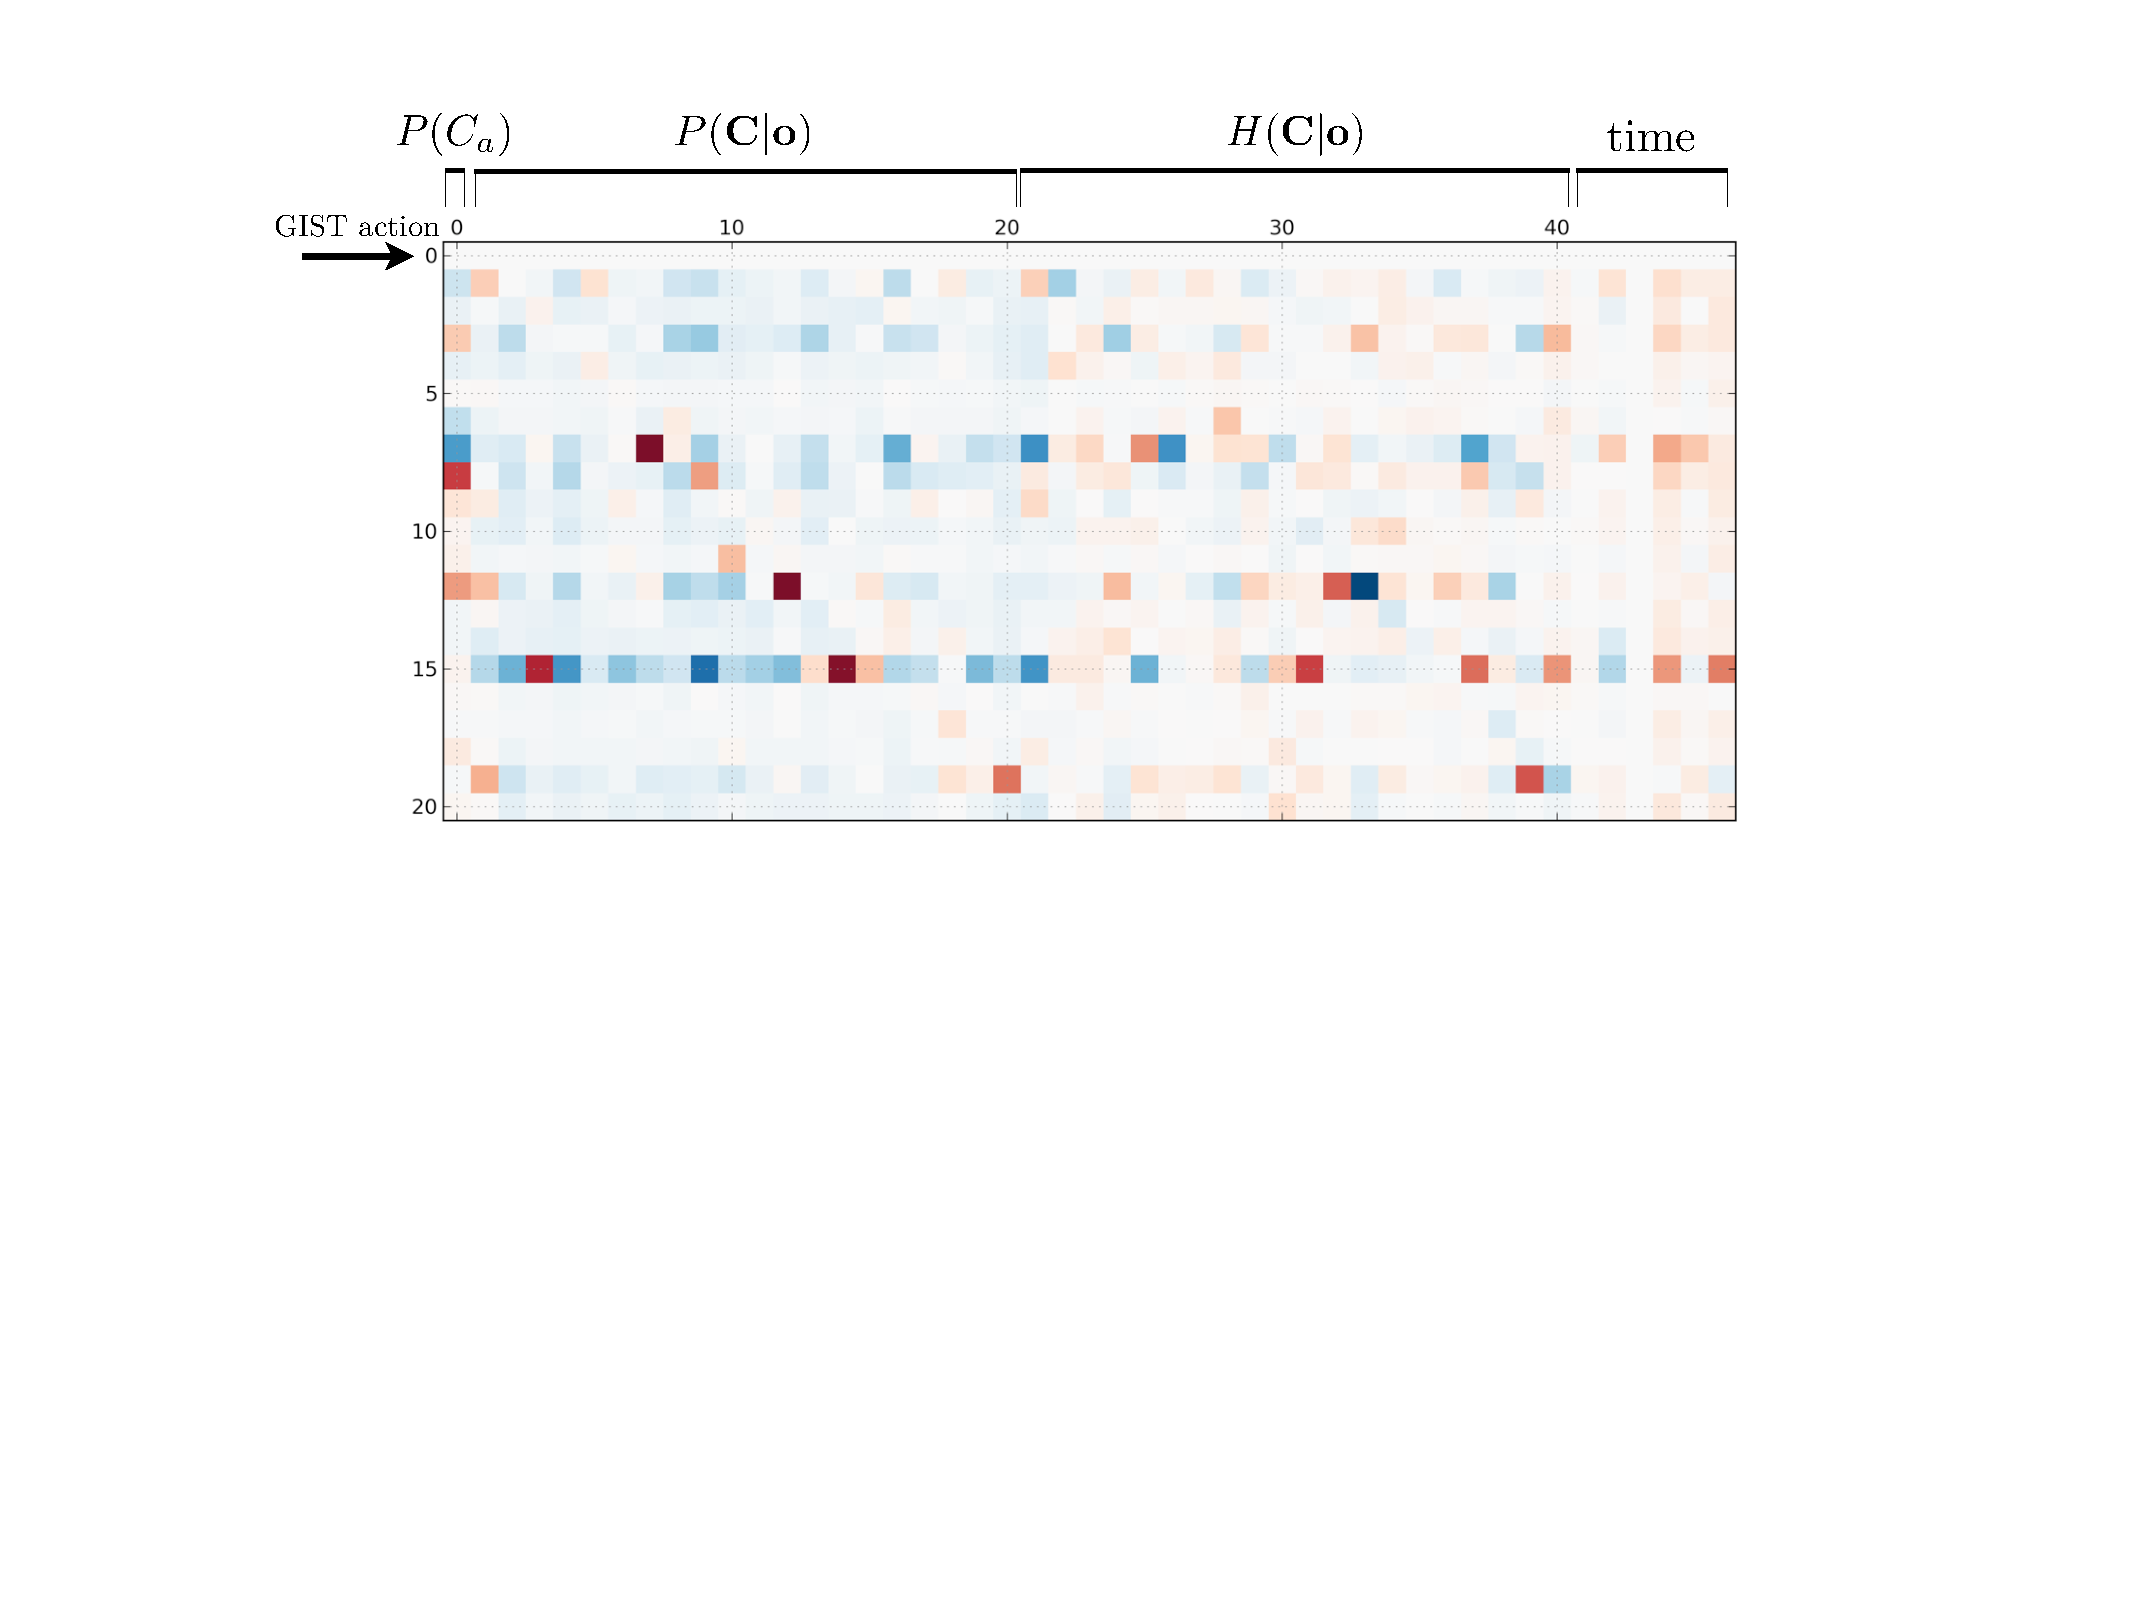
\includegraphics[width=0.49\linewidth]{../figures/weights_greedy}}
\subfloat[RL]{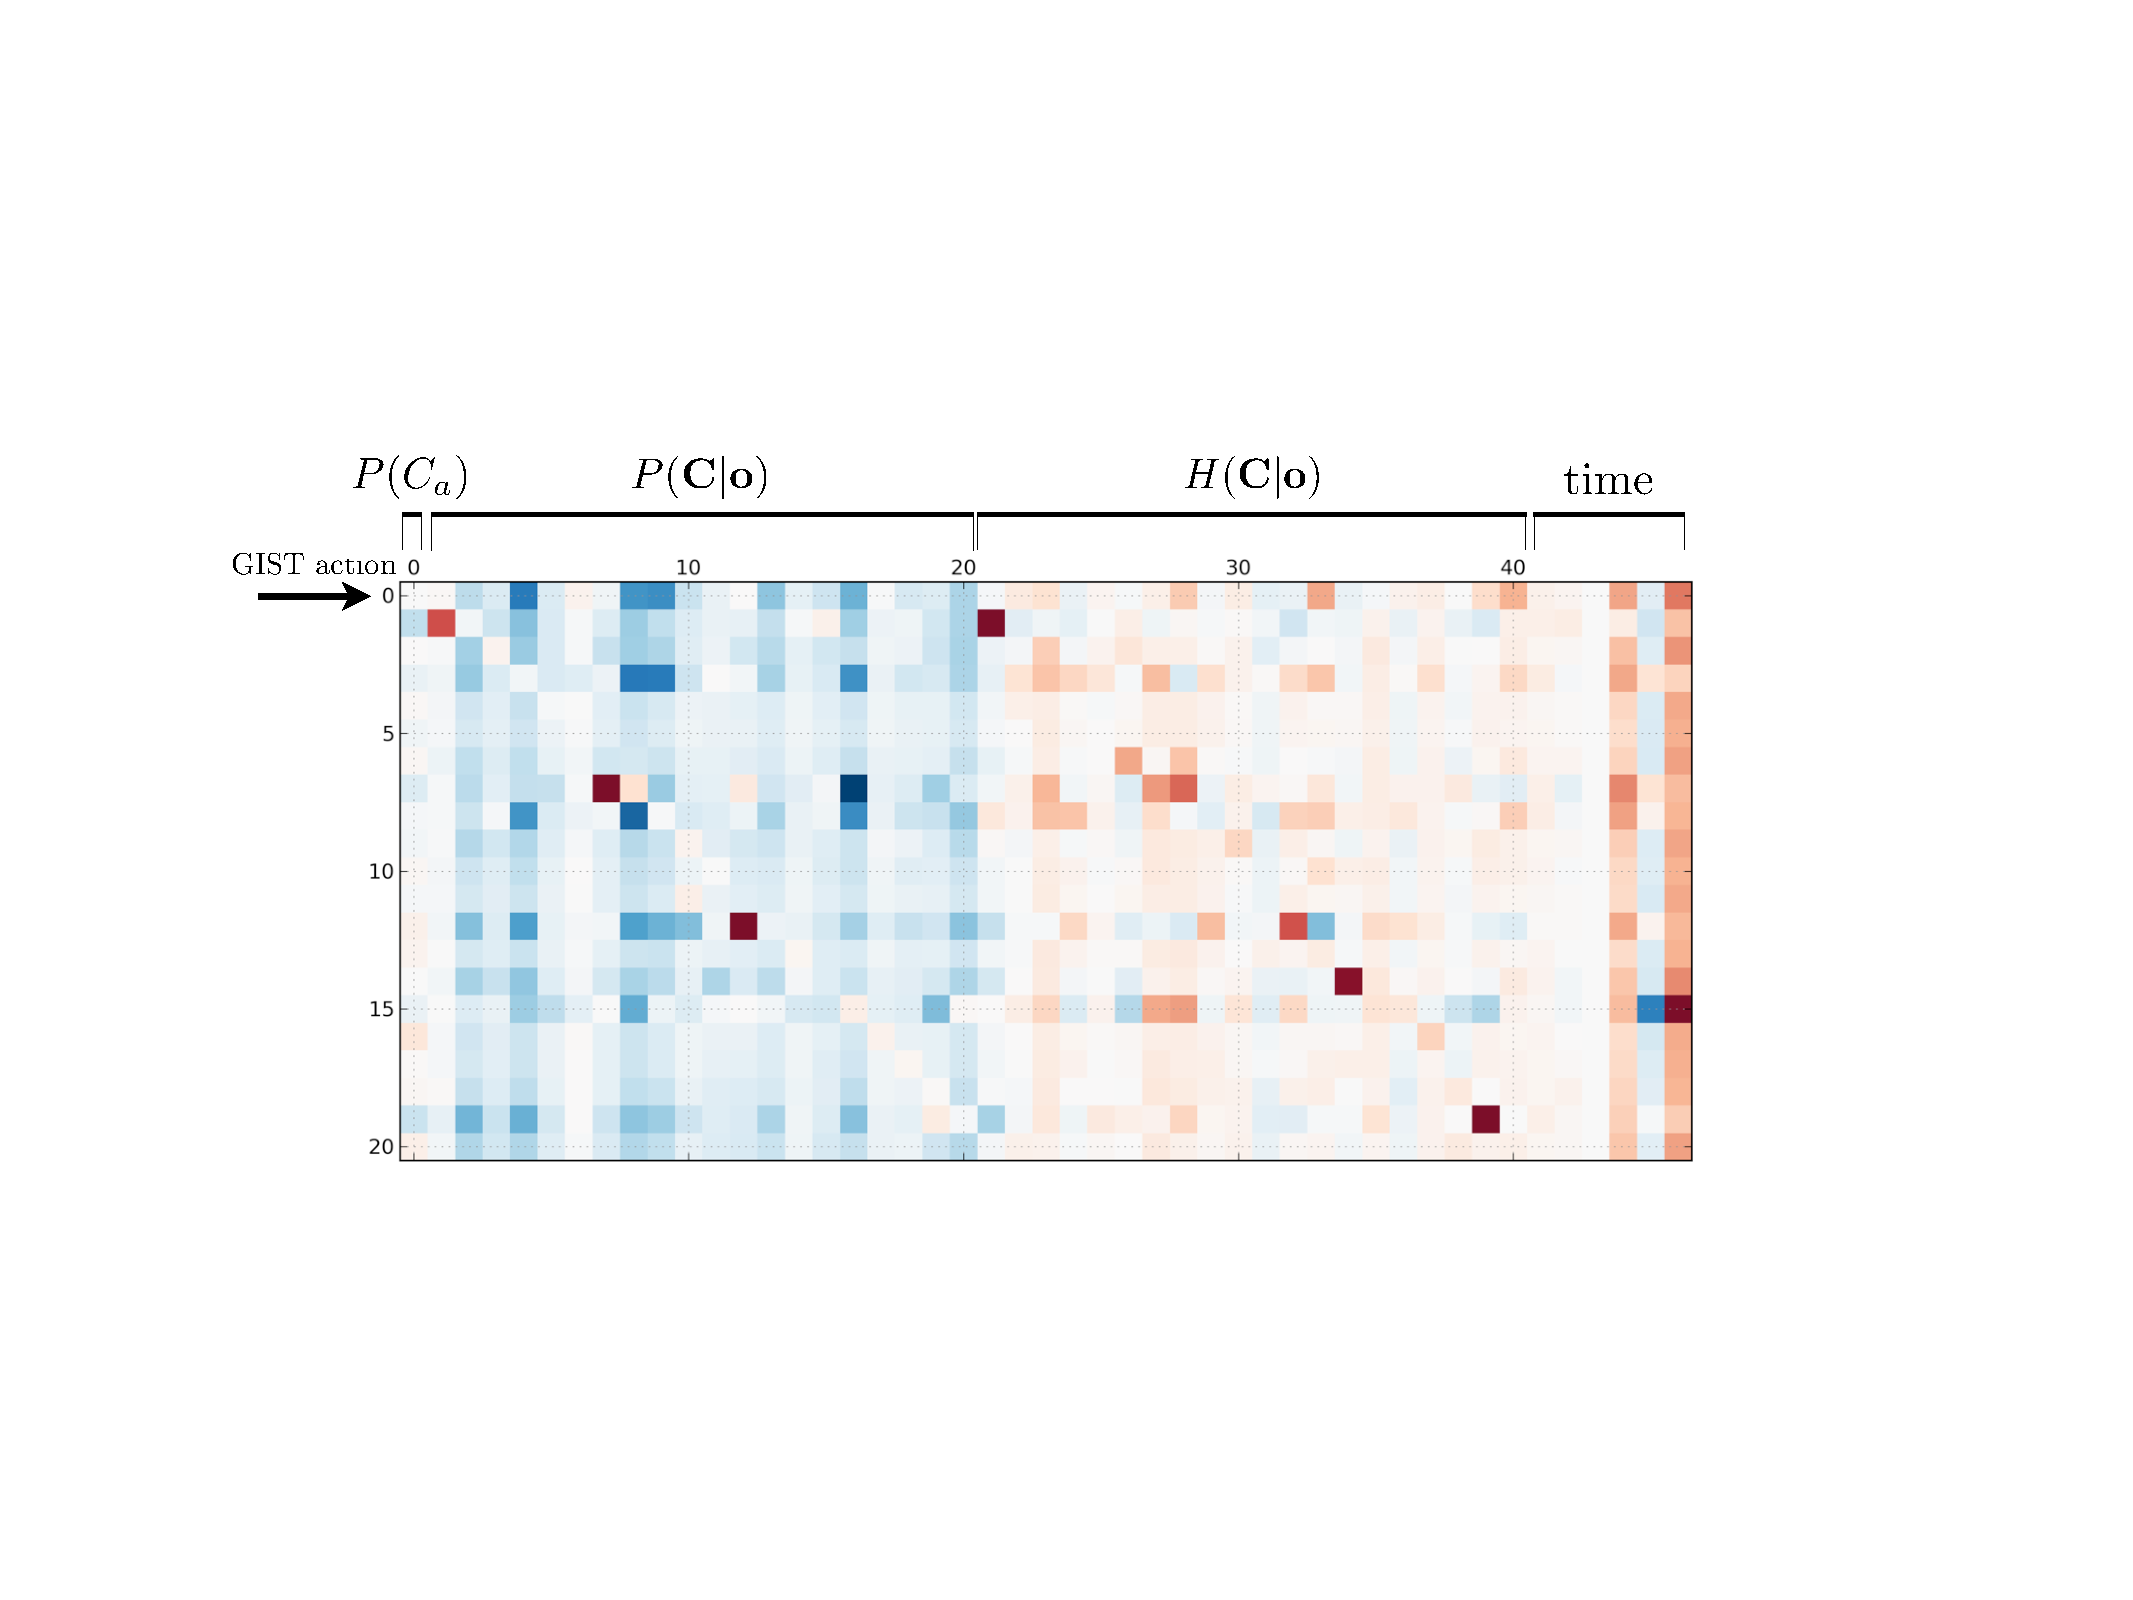
\includegraphics[width=0.49\linewidth]{../figures/weights_rl}}
% 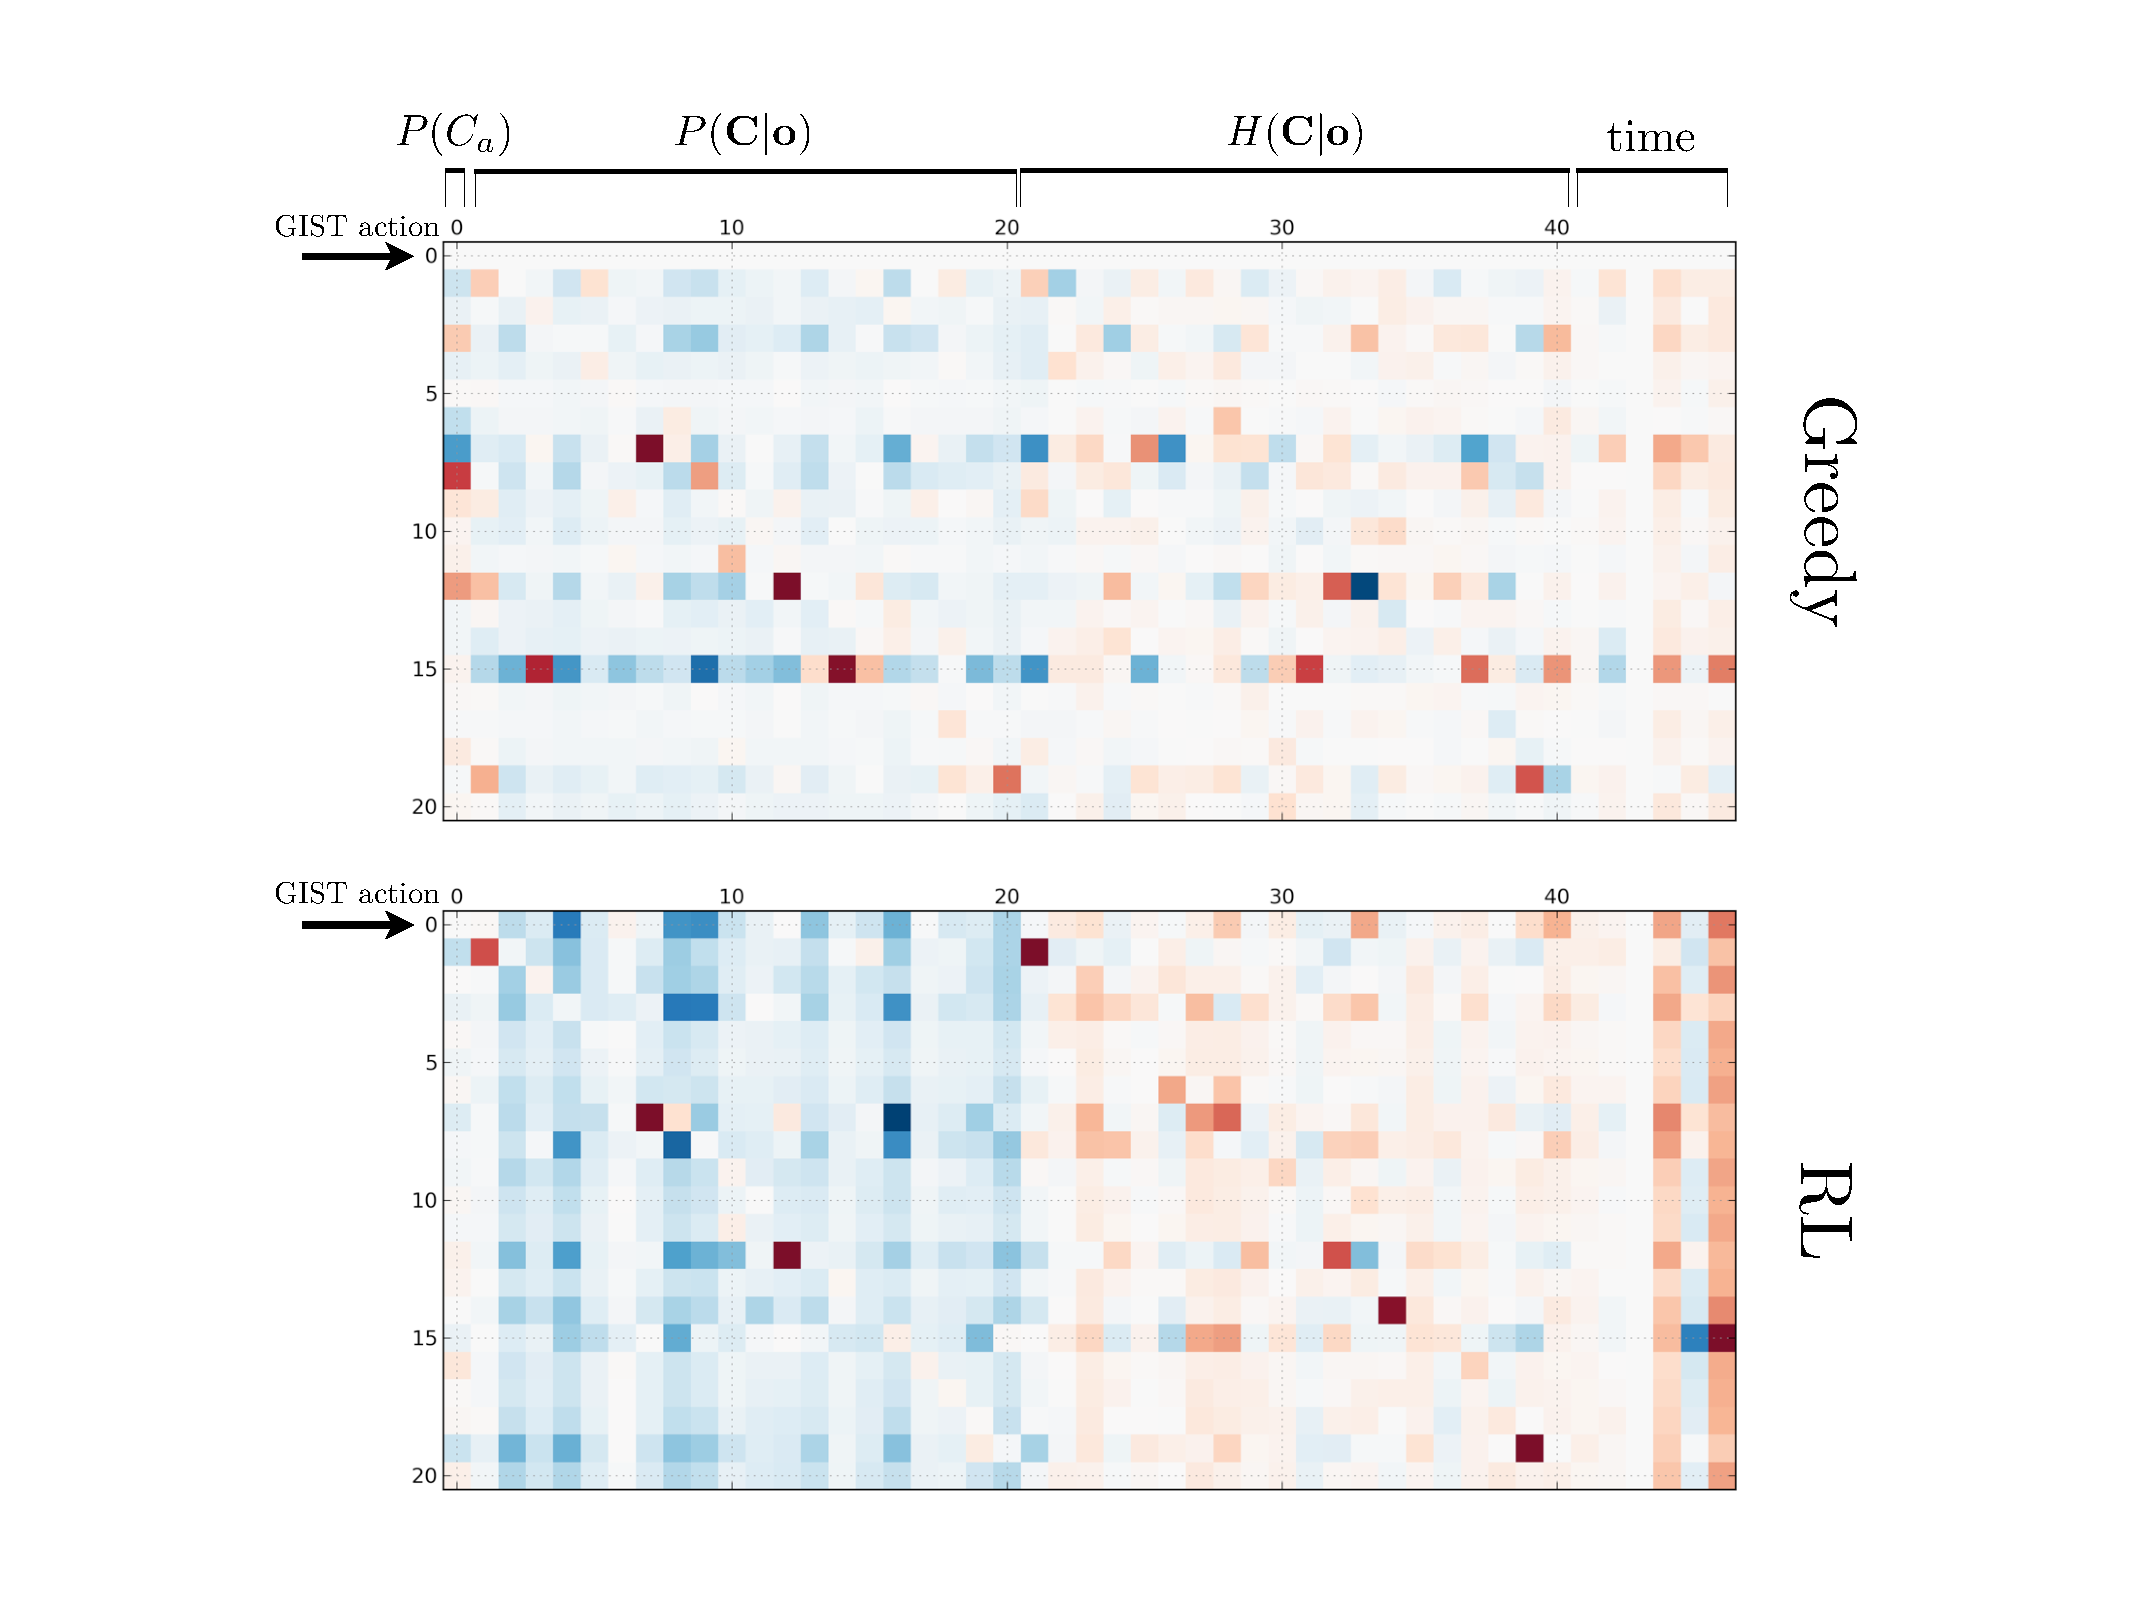
\includegraphics[width=0.87\linewidth]{../figures/weights.pdf}
\caption{
Learned policy weights $\theta_\pi$ (best viewed in color: red corresponds to positive, blue to negative values).
The first row corresponds to the scene-level action, which does not generate detections itself but only helps reduce uncertainty about the contents of the image.
Note that in the greedy learning case, this action is learned to never be taken---whereas it is shown to be useful in the reinforcement learning case.
}
\label{fig:weights}
\end{figure}

\subsection{Updating with observations} \label{sec:updating}

The bulk of our feature representation is formed by probability of individual class occurrence, conditioned on the observations so far: $P(C_0|\mathbf{o}) \ldots P(C_K|\mathbf{o})$.
This allows the action-value function to learn correlations between presence of different classes, and so the policy can look for the most probable classes given the observations.

However, higher-order co-occurrences are not well represented in this form.
Additionally, updating $P(C_i|\mathbf{o})$ presents choices regarding independence assumptions between the classes.

We evaluate two approaches for updating probabilities: \emph{direct} and \emph{MRF}.
In the \emph{direct} method, $P(C_i|\mathbf{o}) = score(C_i)$ if $\mathbf{o}$ includes the observations for class $C_i$ and $P(C_i|\mathbf{o}) = P(C_i)$ otherwise.
This means that an observation of class $i$ does not influence the estimated probability of any class but $C_i$.
$score(C_i)$ for $a_{{det}_i}$ is obtained by training a probabilistic classifier on the detections output.
$score(C_i)$ for $a_{gist}$ is obtained by training probabilistic classifiers on the GIST feature, for all classes.

The \emph{MRF} approach employs a pairwise fully-connected Markov Random Field (MRF), as shown in Figure~\ref{fig:figure1}, with the observation nodes set to $score(C_i)$ appropriately, or considered unobserved.

The graphical model structure is set as fully-connected, but some classes are overwhelmingly unlikely to co-occurr in our dataset.
Accordingly, the graph edge weights are learned with $L_1$ regularization, which obtains the desired sparse structure \cite{Lee2006}.
All parameters of the model are trained on fully-observed data, and Loopy Belief Propagation inference is implemented with an open-source graphical model package \cite{Jaimovich2010}.
% As exact inference is generally intractable in this model, we use Loopy Belief Propagation; although it does not provide general convergence guarantees, it has been shown to work well empirically on similar tasks \cite{Desai2009}.
